In this section, we conduct several experiments on two data sets: (1) the real-world e-commerce apparel data set; (2) the publicly available music data set.  For both data sets, we compare HBayes against several other \emph{state-of-the-art} recommendation methods which are briefly mentioned as follows:

{\noindent\textbf{HSR} \cite{wang2015exploring}: is an item-based recommendation approach that employs a special non-negative matrix factorization for exploring the implicit hierarchical structure of users and items so the user preference towards certain products are better understood.  We adopt HSR  as one baseline. \newline
\textbf{HPF} \cite{gopalan2015scalable}: generates a hierarchical Poisson factorization model for better modeling users' rating towards certain items based upon each one's latent preferences.  Unlike proposed HBayes, HPF does not leverage the content item feature for constructing the hierarchical structure. We adopt HPF as another baseline. \newline
\textbf{SVD++} \cite{mnih2008probabilistic, koren2008factorization}: combines the collaborative filtering approach and latent factor approach, so to provide a more accurate neighboring based recommendation result.  We adopt SVD++ as another baseline. \newline
\textbf{CoClustering} \cite{george2005scalable}: another collaborative filtering type of approach based on weighted co-clustering improvements that simultaneously cluster users and items.  We adopt CoClustering as another baseline. \newline
\textbf{Factorization Machine (FM)} \cite{rendle2010factorization,rendle2012factorization}: combines support vector machines (SVM) with factorization models which takes the advantage of SVM meanwhile overcomes the feature sparsity issues.  In this paper, we adopt LibFM implementation mentioned in \cite{rendle2012factorization} specifically as another baseline. \newline
\textbf{LambdaMART} \cite{burges2010ranknet}: is the boosted tree version of LambdaRank \cite{donmez2009local}, which is based on RankNet \cite{burges2005learning}.  LambdaMART proves to be a very successful approach for ranking as well as recommendation.  We include LambdaMART as another baseline. \newline}

\subsection{Evaluation Metrics}
Throughout the experiments, we compare HBayes against other baselines on the testing held-out data set under the 5-folds cross-validation settings.  For each fold, after fitting the model on the training set, we rank on the test set by each model, and generate the top M samples with maximal ranking scores for recommendation.  Regarding metrics, we adopt precisions and recalls as well as F1-scores for evaluating the product retrieval quality and normalized discounted information gain (NDCG) for the recommendation's ranking quality.  More specifically, precisions, recalls, and F1-scores are defined as follows:

\begin{eqnarray}
\text{Precision@K} & = & \frac{\text{\# of products clicked in top K}}{\text{K}} \nonumber \\
\text{Recall@K}      & = & \frac{\text{\# of products clicked in top K}}{\text{\# of products the user clicked}} \nonumber \\
\text{F1-score@K} & = & 2\cdot\frac{\text{Precision@K} \cdot \text{Recall@K}}{\text{Precision@K} + \text{Recall@K}}  \nonumber
\end{eqnarray}

discounted cumulative gain (DCG) measures the ranking quality based on the item positions from the resulting list, which is defined as follows:
\begin{eqnarray}
\text{DCG@K} & = & \sum_{i=1}^K\frac{r_i}{\log_2(i+1)} =  r_1 + \sum_{i=2}^K\frac{r_i}{\log_2(i+1)}\nonumber
\end{eqnarray}

re-rank all potential products to produce the ideal maximal possible DCG through out first K items, and its corresponding DCG score is called the ideal discounted cumulative gain (IDCG).  By using both DCG and IDCG, the normalized discounted cumulative gain (NDCG) could be defined as follows:

\begin{eqnarray}
\text{NDCG@K} & = & \frac{\text{DCG@K}}{\text{IDCG@K}}\nonumber
\end{eqnarray}

\subsection{Recommendation on Apparel Data}
The first apparel data set is collected from a large e-commerce company.  In this dataset, each sample represents a particular apparel product which is recorded by various features including: categories, titles, and other properties, etc.  Meanwhile, the user click information are also recorded and translated into data labels. Throughout the experiment, positive labels indicate that certain recommended products are clicked by the user, whereas negative samples indicate that the recommended products are skipped by the user which usually implies that the user is `lack of interest' towards that certain item.  By data cleaning and preprocessing of (1) merging duplicated histories; (2) removing users of too few records, the post-processed data set ends up with $\mathbf{895}$ users, $\mathbf{81223}$ products, $\mathbf{5535}$ brands with $\mathbf{380595}$ uniquely observed user-item pairs.  In average, each user has $\mathbf{425}$ products records, ranging from $\mathbf{105}$ to $\mathbf{2048}$, and $\mathbf{61.2\%}$ of the users have fewer than $\mathbf{425}$ product clicking records.  For each item, we encode the popularity and category features into a $\mathbf{20}$ dimensional feature vector; title and product property into a $\mathbf{50}$ dimensional feature vector.  Combining with other features, the total dimension for each sample ends up with $\mathbf{140}$.

\subsubsection{Feature Analysis}
The apparel data are composed of four types of features: (1) product popularity; (2) product category; (3) product title; (4) product properties.  We briefly explain each feature's physical meaning and how we process the data as follows:

\textbf{Product Popularity} (POP): product popularity is a measure of the prevalence of a item in the dataset. In general, consumers have preferences for a particular product during a period of time. This phenomenon is pretty common for apparel products (\emph{e.g.} apparels in certain styles may be of dominant prevalence especially when famous entertainers are wearing them). For a particular product $i$, the popularity is defined as: $\mathrm{\scriptsize POP}_{i} \coloneqq \frac{n_{x_i}}{\mathcal{N}_\mathbf{x}}$, where $n_{x_i}$ are the number of orders or the contribution of gross merchandise volume (GMV) for product $i$,  and $\mathcal{N}_\mathbf{x} = \sum_{\forall x_i}n_{x_i}$ is the summation of $n_{x_i}$ for all such products in the dataset. \newline

\textbf{Product Category} (CID): In e-commerce, items are clustered into different groups based on the alliance/ similarity of the item functionalities and utilities.  In e-commerce websites, such an explicit hierarchy usually exists.  We encode each item's category into a high dimensional vector via one-hot encoding and adjust the feature weights by the popularity of such category. \newline

\textbf{Product Title} (TITLE): product titles are created by vendors and they are typically in the forms of natural languages indicating the product functionality and utility.  Examples could be like `\emph{INMAN short sleeve round neck triple color block stripe T-shirt 2017}'.  We preprocess the product titles by generating the sentence vector embedding based on \cite{de2016representation}.  The main idea is to average the wording weights in the title sentence based on the inverse document frequency (IDF) value of each individual word involved. \newline

\textbf{Product Property Features} (PROP): other product meta data features are also provided in the apparel dataset. For instance, the color feature of items takes value like: `black', `white', `red', etc, and the sizing feature takes value like `S', `M', `L', `XL', etc.  Similar as category features, each product property is first encoded into a binary vector $\bm{x}_i \in \{0, 1\}^{|N|}$, where $N$ denotes the set of all possible corresponding product values.  Then we encode all such property binary vectors into a fixed length ($50$) vector. \newline

On one hand, by utilizing more features HBayes in general reaches better performance in terms of precision-recall metrics.  We report PR-AUC in table (\ref{tab:features_cmp}) to prove this argument; on the other hand, more features needs much more training time.  Figure (\ref{fig:train_time_cmp}) reports the changes in likelihood against training time cost (in minutes) for each feature use cases\footnote{The experiment is conducted via the same Linux Qual core 2.8 GHz Intel Core i7 macbook with 16 Gigabytes of memory}. It is shown that by only taking POP features, model spends less than 5 minutes to converge while taking POP+CID+TITLE+PROP features, the model needs more than 6 hours in training.   

\begin{table}[htb]
\centering
\scalebox{0.85}{
\begin{tabular}{l|c}
\toprule
\textbf{Features} & \textbf{PR AUC} \\
\hline
POP & 0.0406 \\
\rowcolor{mygray}
POP+CID & 0.0414 \\
POP+CID+TITLE & 0.0489 \\
\rowcolor{mygray}
POP+CID+TITLE+PROP & 0.0491 \\
\bottomrule
\end{tabular}}
\caption{Model performance under different feature combinations in terms of PR AUC}
\label{tab:features_cmp}
\end{table}

\begin{figure*}[!htb]
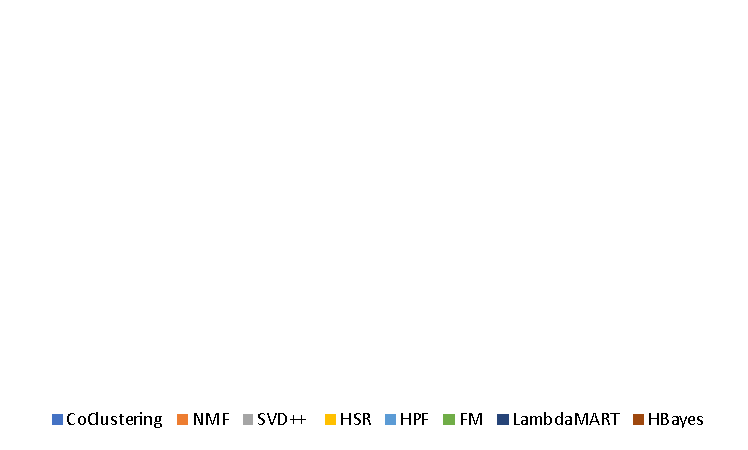
\includegraphics[width=0.7\linewidth]{fig/legend}
\end{figure*}

\begin{figure*}[!htb]
\minipage{0.32\textwidth}
  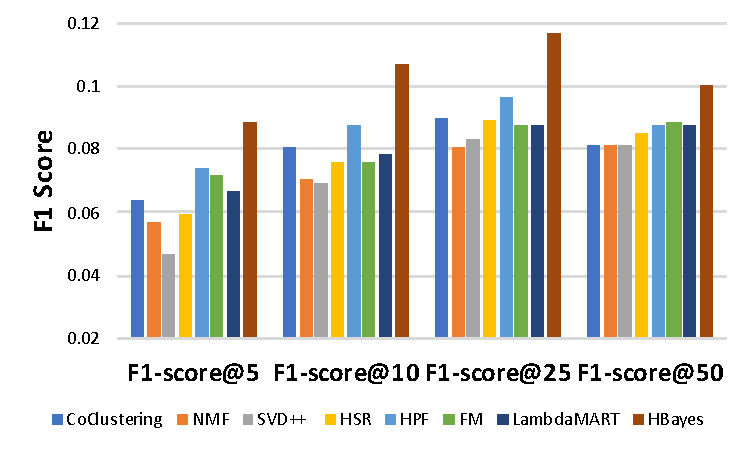
\includegraphics[width=\linewidth]{fig/F1-score_jd}
  \caption{F1@K on \emph{Apparel} data.}
  \label{fig:perf_cmp_F1_apparel}
\endminipage\hfill
\minipage{0.32\textwidth}
  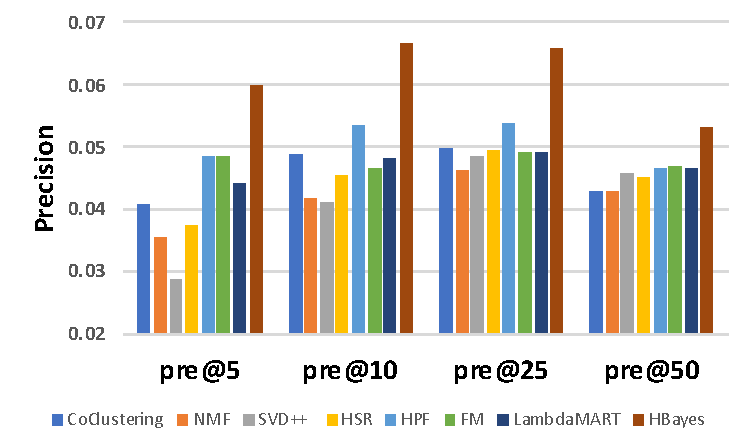
\includegraphics[width=\linewidth]{fig/precision_jd}
  \caption{Precision@K on \emph{Apparel} data.}
  \label{fig:perf_cmp_precision_apparel}
\endminipage\hfill
\minipage{0.32\textwidth}%
  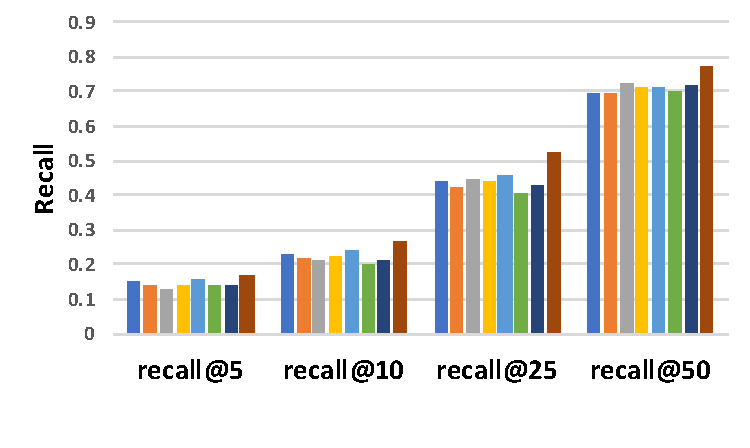
\includegraphics[width=\linewidth]{fig/recall_jd}
  \caption{Recall@K on \emph{Apparel} data.}
  \label{fig:perf_cmp_recall_apparel}
\endminipage
\end{figure*}


\begin{figure*}[!htb]
\minipage{0.32\textwidth}
  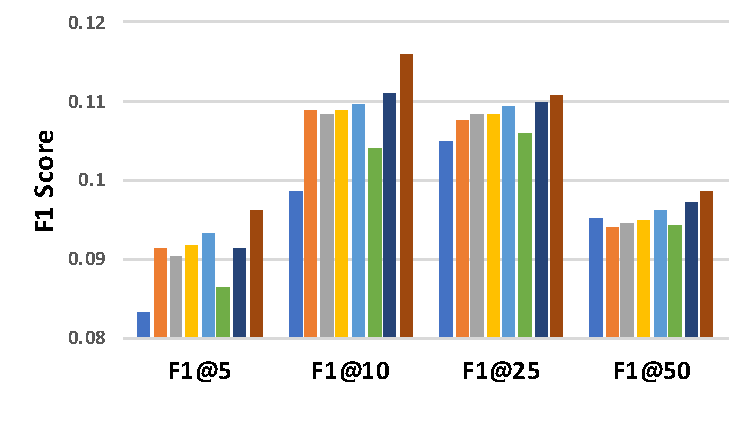
\includegraphics[width=\linewidth]{fig/F1-score_music}
  \caption{F1@K on \emph{Music} data.}
  \label{fig:perf_cmp_F1_music}
\endminipage\hfill
\minipage{0.32\textwidth}
  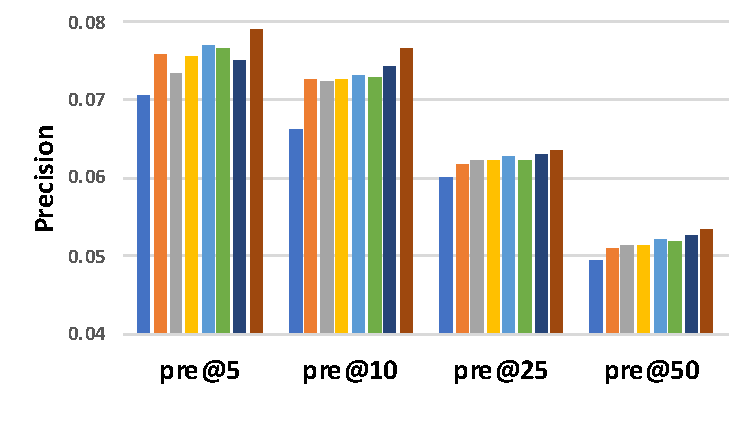
\includegraphics[width=\linewidth]{fig/precision_music}
  \caption{Precision@K on \emph{Music} data.}
  \label{fig:perf_cmp_precision_music}
\endminipage\hfill
\minipage{0.32\textwidth}%
  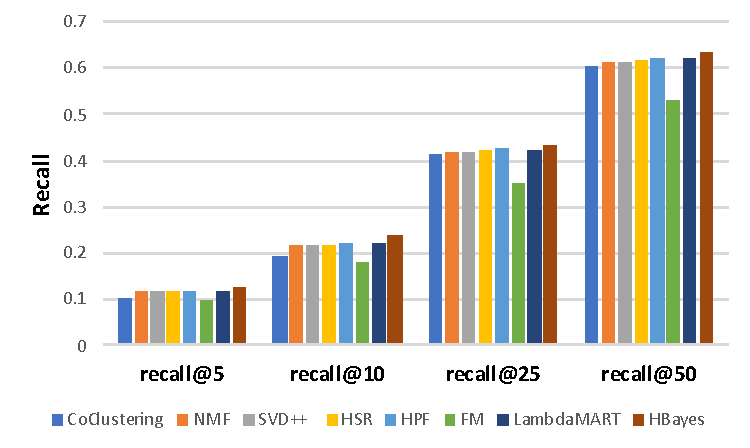
\includegraphics[width=\linewidth]{fig/recall_music}
  \caption{Recall@K on \emph{Music} data.}
  \label{fig:perf_cmp_recall_music}
\endminipage
\end{figure*}

\begin{figure}[!htb]
\centering
\minipage{0.49\columnwidth}
  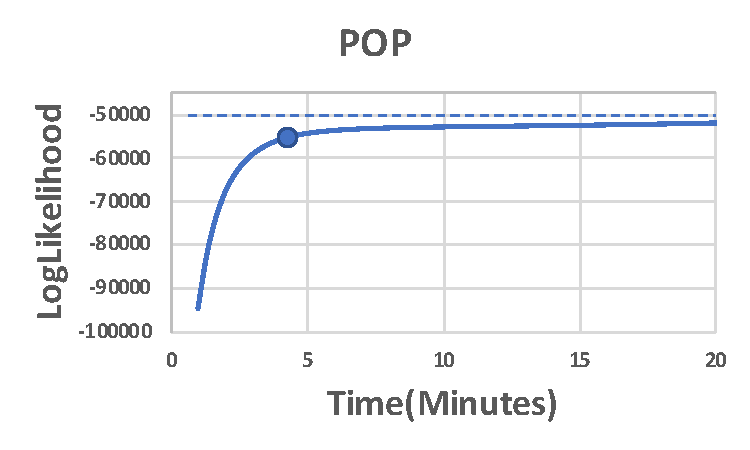
\includegraphics[width=\linewidth]{fig/1feature_lik}
\endminipage
\minipage{0.49\columnwidth}
  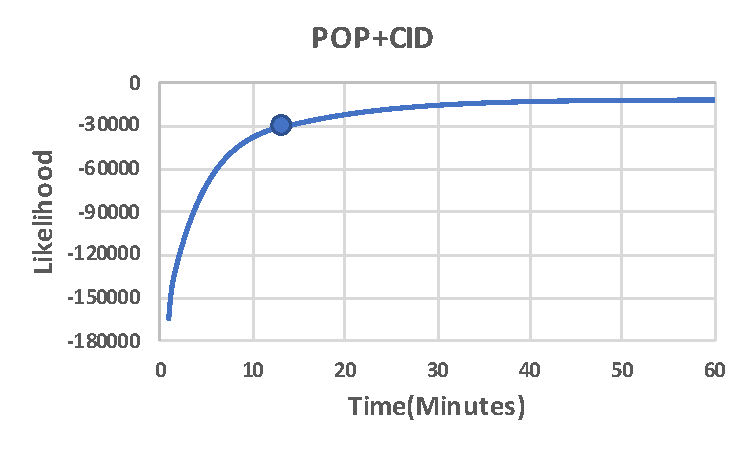
\includegraphics[width=\linewidth]{fig/2feature_lik}
\endminipage
\vskip\baselineskip
\minipage{0.49\columnwidth}
  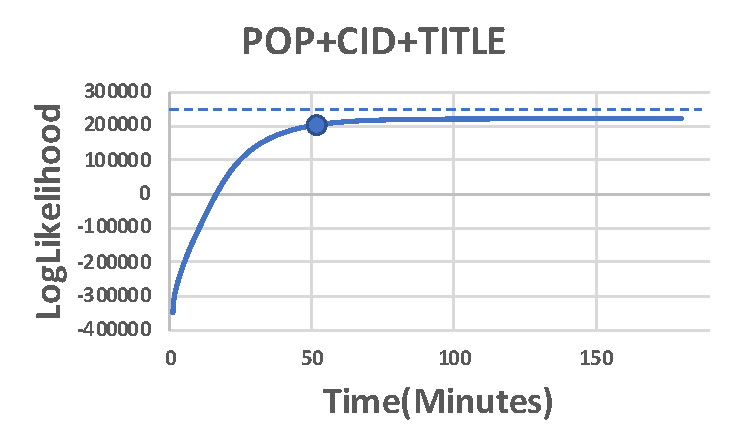
\includegraphics[width=\linewidth]{fig/3feature_lik}
\endminipage
\minipage{0.49\columnwidth}
  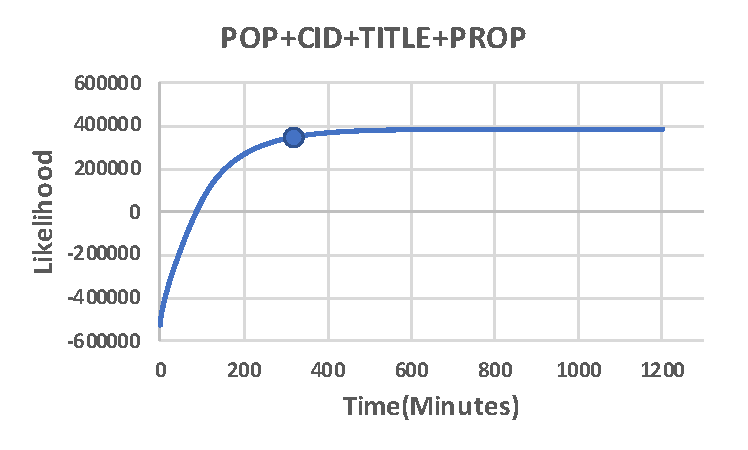
\includegraphics[width=\linewidth]{fig/4feature_lik}
\endminipage
\caption{Training time under different feature combinations on e-commerce recommendations}
\label{fig:train_time_cmp}
\end{figure}

%\begin{figure}[htb]
%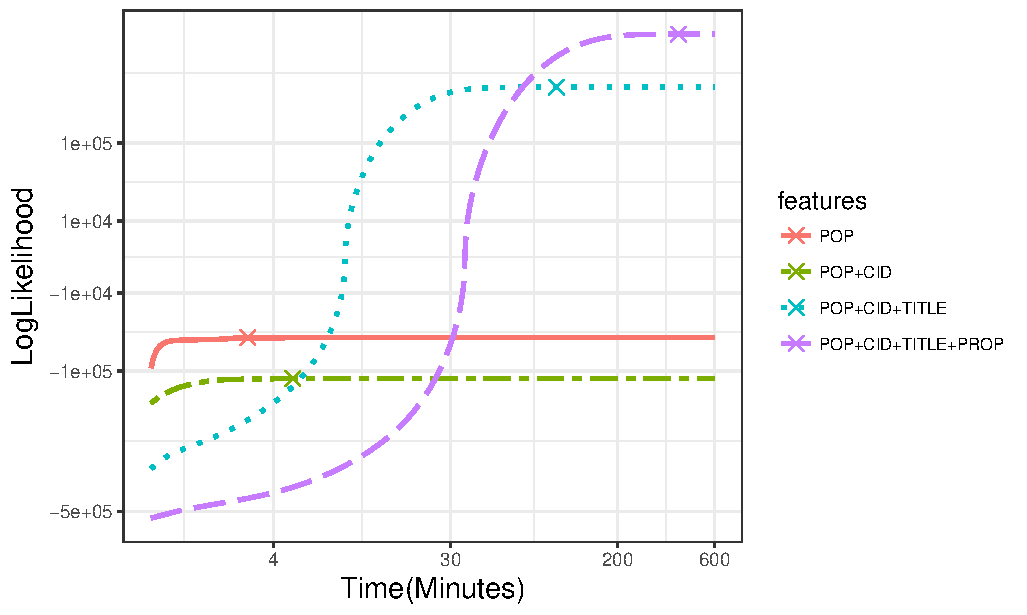
\includegraphics[width=0.9\columnwidth,height=0.5\columnwidth]{fig/Lik_time}
%\caption{Training time under different feature combinations on e-commerce recommendations}
%\label{fig:train_time_cmp}
%\end{figure}

\begin{table}[htb]
\begin{center}
\scalebox{0.85}{
\begin{tabular}{l|cccc}
\toprule
\textbf{Method} & \textbf{NDCG@5} & \textbf{NDCG@10} & \textbf{NDCG@25} & \textbf{NDCG@50} \\
\hline
\rowcolor{mygray}
CoClustering & 0.1288 & 0.1637 & 0.2365 & 0.3050 \\
NMF & 0.1249 & 0.0156 & 0.2272 & 0.3020 \\
\rowcolor{mygray}
SVD++ & 0.1138 & 0.1487 & 0.2287 & 0.3073\\
HSR & 0.1266 & 0.1603 & 0.2354 & 0.3107 \\
\rowcolor{mygray}
HPF & 0.1412 & 0.1757 & 0.2503 & 0.3229 \\
FM & 0.1363 & 0.1592 & 0.2291 & 0.3117\\
\rowcolor{mygray}
LambdaMART & 0.1287 & 0.1585 & 0.2304 & 0.3123\\
HBayes & \textbf{0.1557} & \textbf{0.1974} & \textbf{0.2871} & \textbf{0.3590}\\
\bottomrule
\end{tabular}}
\end{center}
\caption{NDCG on apparel recommendations}
\label{NDCG_cmp}
\end{table}

\subsubsection{Performance Comparison}
We first report the model performance regarding precision, recall, as well as F1-score for HBayes against other baselines in Figure (\ref{fig:perf_cmp_F1_apparel},\ref{fig:perf_cmp_precision_apparel},\ref{fig:perf_cmp_recall_apparel}).  As shown when each method recommend fewer number of products (K = 5), HBayes does not show the superiority regarding with recalls, with the increment of recommended items, the recall for HBayes becomes much better against others, which implies HBayes is really efficient in terms of finding items that people tend to take interest in.  In the sense of precision, HBayes is consistently better than other baseline methods which implies HBayes is much more accurate in terms of item classification.   Given the performance of precisions and recalls, HBayes is much better regarding F1-score with different K for apparel recommendation.

Regarding the ranking quality, we use NDCG to report each method's performance in Table (\ref{NDCG_cmp}).  HBayes is superior against other baseline methods through out different K recommended.  Specially, HBayes beats the second best HPF at $\text{K}=5$ by $10.3\%$, at $\text{K}=10$ by $12.4\%$, at $\text{K}=25$ by $14.7\%$ and at $\text{K}=50$ by $11.2\%$.  

\subsubsection{Model Learning Analysis}
\begin{figure}
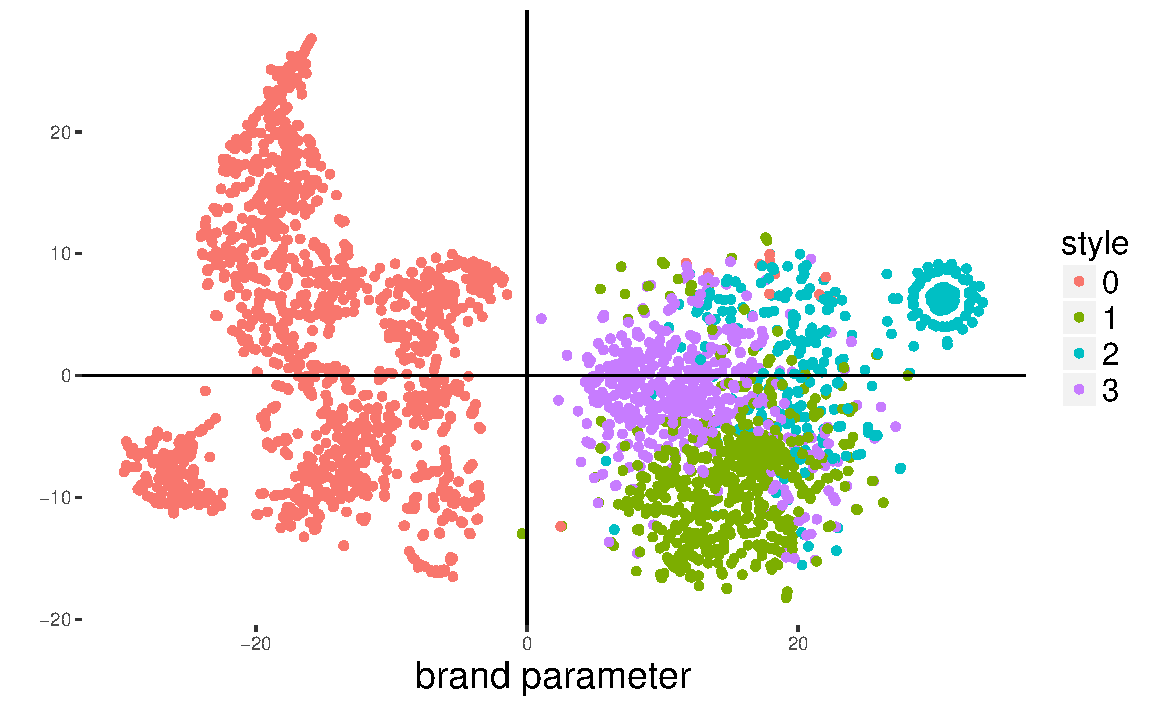
\includegraphics[width=0.58\columnwidth,height=3cm]{fig/brand_tsne}
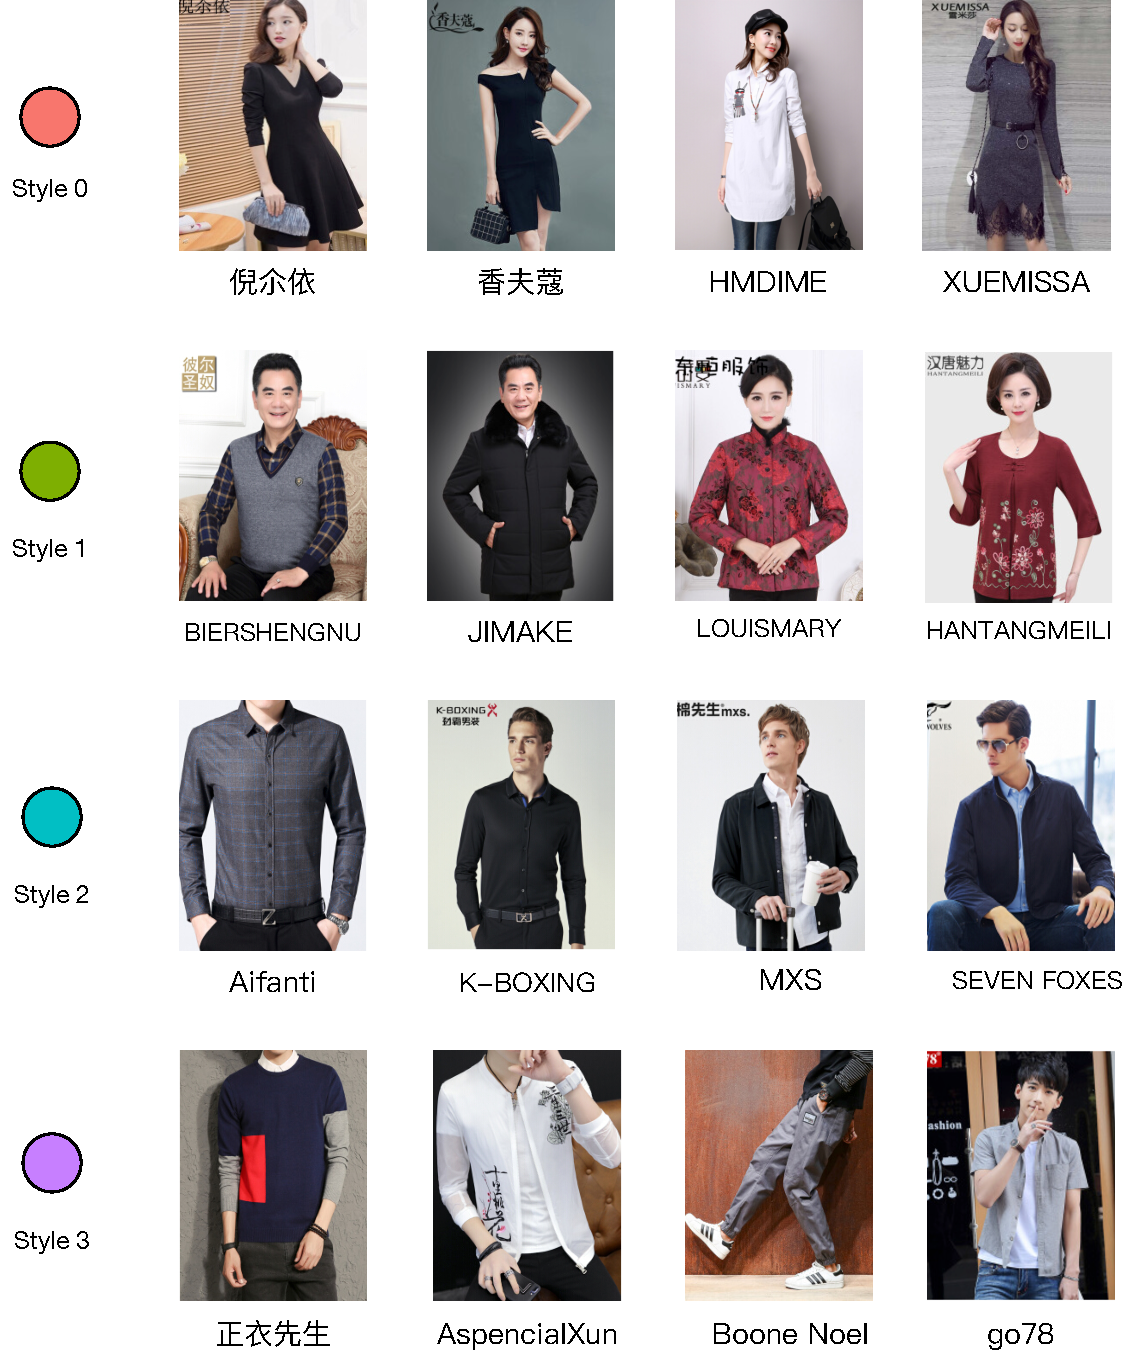
\includegraphics[width=0.39\columnwidth,height=4cm]{fig/style-brand}
\caption{tSNE of four latent apparel style clusters}
\label{fig:tsne-represntation-style-cluster}
\end{figure}

Like mentioned in Sec.\ref{sec:method}, HBayes learns the latent style clusters, and group different brands of products based on their different hidden style representations.  Figure (\ref{fig:tsne-represntation-style-cluster}) shows the tSNE \cite{maaten2008visualizing} representations for different apparel clusters learned by HBayes and we randomly pick $4$ samples out of each cluster and display their product images at the right subfigure.  As shown, cluster one taking the majority proportion of apparel items seems about stylish female youth garment.  This intuitively makes sense since the majority of apparel customers are female youth for e-commerce websites; as a result, most apparels are also focusing on female customer audience.    The second cluster seems about senior customers who are elder in age.   Interestingly, the third cluster and the fourth cluster which are closely tied up are both about male customer youth.  However, the third cluster seems focusing more on office business garment while the fourth cluster seems more about K-pop street styles.  This indicates us that the HBayes indeed learns the meaningful intrinsic garment styles from apparel items by leveraging customer behavior data.   

\subsection{Recommendation on Last.fm Music Data}
The second data set is collected from Last.fm dataset \cite{Celma:Springer2010} and Free Music Archive (FMA) \cite{FMA}. Last.fm is a publicly available dataset which contains the whole listening habits (till May, 5th 2009) for $\mathbf{1000}$ users. FMA is an open and easily accessible dataset providing $\mathbf{917}$ GiB and $\mathbf{343}$ days of Creative Commons-licensed audio from $\mathbf{106574}$ tracks, $\mathbf{16341}$ artists and $\mathbf{14854}$ albums, arranged in a hierarchical taxonomy of $\mathbf{161}$ genres. It also provides full-length and high quality audios with precomputed features.  In our experiment, tracks in Last.fm dataset were further intersected with FMA dataset for better feature generation.  The resulting dataset contains $\mathbf{500}$ users, $\mathbf{16328}$ tracks and $\mathbf{36}$ genres.

\subsubsection{Performance Comparison}
We conduct similar experiments as we do for apparel data set and report precisions, recalls as well as F1-scores in Figure (\ref{fig:perf_cmp_F1_music},\ref{fig:perf_cmp_precision_music},\ref{fig:perf_cmp_recall_music}).  Although HPF and HBayes share similar performance regarding recalls along with different K, HBayes is dominant for precision at different K, specially when K is small (5, 10), which indicates HBayes is very efficient and precise for helping users pick up the songs they prefer even when the recommended item lists are short.   Combining the two, HBayes is superior in F1-scores for different K recommended.  

In terms of ranking quality, we report the NDCG performance in Table (\ref{NDCG_cmp_music}).  Similar as e-commerce apparel data, HBayes is the best approach and HPF is the second best one throughout different K items recommended.  Specifically, HBayes beats HPF for $2.7\%$ at $\text{K}=5$, $4.3\%$ at $\text{K}=10$, $2.1\%$ at $\text{K}=25$, and $2.5\%$ at $\text{K}=50$ separately.

\begin{table}[htb]
\begin{center}
\scalebox{0.85}{
\begin{tabular}{l|cccc}
\toprule
\textbf{Method} & \textbf{NDCG@5} & \textbf{NDCG@10} & \textbf{NDCG@25} & \textbf{NDCG@50} \\
\hline
\rowcolor{mygray}
CoClustering & 0.2415 & 0.2314 & 0.2289 & 0.2349 \\
NMF & 0.2556 & 0.2494 & 0.2368 & 0.2431 \\
\rowcolor{mygray}
SVD++ & 0.2493 & 0.2478 & 0.2381 & 0.2439\\
HSR & 0.2544 & 0.2495 & 0.2384 & 0.2448\\
\rowcolor{mygray}
HPF & 0.2584 & 0.2513 & 0.2405 & 0.2474\\
FM & 0.2527 & 0.2453 & 0.2284 & 0.2333\\
\rowcolor{mygray}
LambdaMART & 0.2372 & 0.2337 & 0.2272 & 0.2218\\
HBayes & \textbf{0.2655} & \textbf{0.2620} & \textbf{0.2455} & \textbf{0.2537}\\
\bottomrule
\end{tabular}}
\caption{NDCG on Last.fm recommendations}
\label{NDCG_cmp_music}
\end{center}
\end{table}

%For PR-AUC, HBayes (0.055) again beats against the second best, which is LambdaMART (0.043) by $27.9\%$.  In terms of F1-score, HBayes in average beats against LambdaMART by $14.0\%$.  Regarding with the ranking quality, HBayes beats against the second best, which is NMF  for $M=5,10,25$ by $4.20\%$ in average and SVD++ for $M=50$ by $4.02\%$.  









